\documentclass{article}
\usepackage{enumerate}
\usepackage{amsmath}
\usepackage{amssymb}
\usepackage{graphicx}
\usepackage{subfigure}
\usepackage{geometry}
\usepackage{caption}
\usepackage{stmaryrd}
\geometry{left=3.0cm,right=3.0cm,top=3.0cm,bottom=4.0cm}
\renewcommand{\thesection}{Problem \arabic{section}.}
\title{VP260 PROBLEM SET 9}
\author{Liu Yihao 515370910207}
\date{}
\begin{document}
\maketitle

\section{}
\begin{enumerate}[(a)]
\item
$$\overline{E}=0$$
According to Maxwell's equations,
$${\rm rot\ }\overline{E}=-\frac{\partial\overline{B}}{\partial t}=0$$
$$\frac{\partial\overline{B}}{\partial t}=0$$
\item
According to Maxwell's equations,
$$\oint_r\overline{E}d\bar{l}=-\frac{d\Phi_B}{dt}=0$$
So $\Phi_B$ is a constant.
\end{enumerate}

\section{}
$$\overline{B}=0$$
According to Maxwell's equations,
$$\oint_r\overline{B}d\bar{l}=\mu_0i+\mu_0\epsilon_0\frac{d\Phi_E}{dt}=0$$
Since $\overline{E}=0$ according to Problem 1, we can simply get
$$i=0$$
inside the conductor. So the electric current is confined to the surface.

\section{}
In picture (A),
$$\varepsilon_1=\varepsilon_2=\frac{\varepsilon}{2}=-\frac{1}{2}\frac{d\Phi_B}{dt}$$
In picture (B), in the loop containing the bulb in the bottom,
$$d\Phi_B=0,\varepsilon_2=0$$
So the bulb in the bottom no longer glows.\\
In the loop containing the bulb above,
$$\varepsilon_1=\varepsilon=-\frac{d\Phi_B}{dt}$$
Since $\varepsilon_{B1}=2\varepsilon_{A1}$, the top bulb gets much brighter.

\section{}
$$\varepsilon=-\frac{d\Phi_B}{dt}=-\alpha$$
$$I=\frac{\varepsilon}{R_1+R_2}=-\frac{\alpha}{R_1+R_2}$$
So the direction of $I$ is clockwise.
According to the connection direction of $V_1$ and $V_2$,
$$V_1=-IR_1=\frac{\alpha R_1}{R_1+R_2}$$
$$V_2=IR_2=-\frac{\alpha R_2}{R_1+R_2}$$

\section{}
$$\varepsilon_1=-N_1\frac{d\Phi_B}{dt}$$
$$\varepsilon_2=-N_2\frac{d\Phi_B}{dt}$$
$$\frac{\varepsilon_2}{\varepsilon_1}=\frac{N_2}{N_1}$$

\section{}
$$L_1\frac{dI_1}{dt}+M\frac{dI_2}{dt}=U$$
$$L_2\frac{dI_2}{dt}+M\frac{dI_1}{dt}=U$$
$$\frac{dI_1}{dt}=\frac{U-M\frac{dI_2}{dt}}{L_1}$$
$$L_2\frac{dI_2}{dt}+M\frac{U-M\frac{dI_2}{dt}}{L_1}=U$$
$$\frac{dI_2}{dt}=\frac{L_1-M}{L_1L_2-M^2}U$$
$$\frac{dI_1}{dt}=\frac{L_2-M}{L_1L_2-M^2}U$$
$$\frac{dI}{dt}=\frac{dI_1}{dt}+\frac{dI_2}{dt}=\frac{L_1+L_2-2M}{L_1L_2-M^2}U$$
$$L=\frac{L_1L_2-M^2}{L_1+L_2-2M}$$

\section{}
\begin{enumerate}[(a)]
\item
$$L=\frac{d\Phi_B}{dt}=\mu_0N\pi a^2l$$
$$L_1=\mu_0N_1\pi a^2l,L_2=\mu_0N_2\pi a^2l$$
$$M=\mu_0\pi a^2N_1N_2l$$
$$M^2=L_1L_2$$
\item
$$\varepsilon_2=-M\frac{dI_2}{dt}$$
$$U_1=-L_1\frac{dI_1}{dt}$$
$$-M\frac{dI_2}{dt}-L_1\frac{dI_1}{dt}+V_1\cos\omega t=0$$
$$M\frac{dI_2}{dt}+L_1\frac{dI_1}{dt}=V_1\cos\omega t$$
$$\varepsilon_2=-M\frac{dI_1}{dt}$$
$$U_2=-L_2\frac{dI_2}{dt}$$
$$-M\frac{dI_1}{dt}-L_2\frac{dI_2}{dt}-I_2R=0$$
$$M\frac{dI_1}{dt}+L_2\frac{dI_2}{dt}=-I_2R$$
\item
$$\frac{dI_2}{dt}=-\frac{I_2R+M\frac{dI_1}{dt}}{L_2}$$
$$-M\frac{I_2R+M\frac{dI_1}{dt}}{L_2}+L_1\frac{dI_1}{dt}=V_1\cos\omega t$$
$$I_2=-\frac{V_1L_2\cos\omega t}{MR}$$
$$L_1I_1+MI_2=\int V_1\cos\omega t$$
$$I_1=\frac{V_1}{L_1\omega}\sin\omega t+\frac{V_1L_2}{L_1R}\cos\omega t$$
\item
$$V_{out}=I_2R=-\frac{V_1L_2\cos\omega t}{M}$$
$$\frac{V_{out}}{V_{in}}=\frac{L_2}{M}=\frac{\sqrt{L_2}}{\sqrt{L_1}}=\frac{N_2}{N_1}$$
\item
$$P_{in}=V_{in}I_1=\frac{V_1^2}{L_1\omega}\sin\omega t\cos\omega t+\frac{V_1^2L_2}{L_1R}\cos^2\omega t$$
$$\overline{P_{in}}=\frac{1}{2\pi}\int_0^{2\pi}P_{in}=\frac{V_1^2L_2}{2L_1R}$$
$$P_{out}=I_2^2R=\frac{V_1^2L_2^2\cos^2\omega t}{M^2R}$$
$$\overline{P_{out}}=\frac{1}{2\pi}\int_0^{2\pi}P_{out}=\frac{V_1^2L_2^2}{2M^2R}$$
$$\frac{V_1^2L_2}{2L_1R}=\frac{V_1^2L_2^2}{2M^2R}$$
So they are equal.
\end{enumerate}

\section{}
\begin{enumerate}[(a)]
\item
Since the current in the inductor can't change suddenly and the capacitor can be seen as a open circuit,
$$I_1=I_3=\frac{40}{50}=0.8A, I_2=I_4=0A$$
$$U_1=40V,U_2=U_3=U_4=U_5=0V$$
\item
Since the inductor can be seen as a short circuit, 
$$R=50+\frac{1}{1/50+1/100}=\frac{250}{3}\Omega$$
$$I_1=\frac{40}{250/3}=0.48A,I_2=0.48\cdot\frac{50}{150}=0.16A,I_3=0.32A,I_4=0A$$
$$U_1=40\cdot\frac{50}{250/3}=24V,U_2=0V,U_3=U_4=U_5=16V$$
\item
$$Q=CV=12\times10^{-6}\cdot16=1.92\times10^{-4}C$$
\item \ 
\begin{figure}[h]
	\centering
	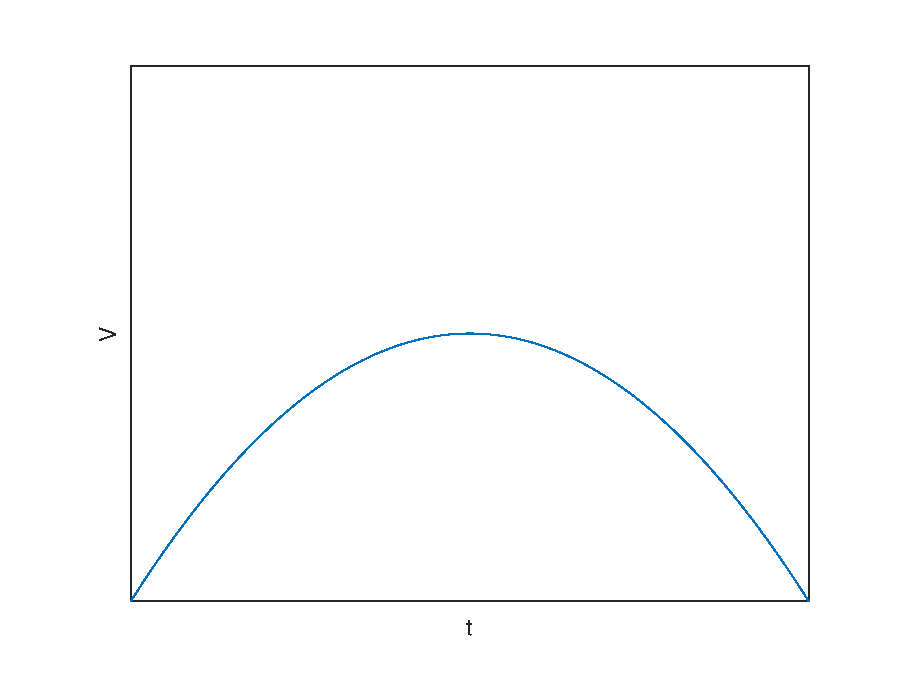
\includegraphics[scale=0.4]{1.eps}
\end{figure}
\end{enumerate}


\end{document}
